\section{Regular Expressions and Finite State Machine}

Regular expressions and Finite Automata (FA) represent a valuable concept in theoretical computer science. Their equivalence is well known dating back to the Kleen's paper in 1956. REs are well suited for human users and therefore often used as interfaces to specify certain patterns or languages, while automata immediately translate to efficient data structures and are suited for programming tasks. Obviously this fact raises the interest in conversion algorithms between them ~\cite{refa}. 

Moreover, when reasoning about the specifications of properties for RV, it can be useful to convert between them and observe how changes in one of the specifications are reflected in the other. That was the main motivation for use Bidirectional Transformations between these two types of specifications.

The next sections will describe some formal definitions of RE and FA as well as the known algorithms to convert between them. 

\subsection{Formal definitions}
\label{definitions}
Before introduce the known algorithms for conversion it is useful to present and formally describe the two types of automata. 

\subsubsection{Regular Expressions} 
Given a vocabulary $\Sigma$, a symbol $a \in \Sigma$ and the regular expressions $s$ and $t$, then RE can be defined inductively as following: 

\begin{equation*}
    RE = \quad \emptyset \quad | \quad \epsilon \quad | \quad a \quad | \quad (s+t) \quad | \quad (s\ .\ t) \quad | \quad (s)^*
\end{equation*}

The language defined by a regular expression $r$, denoted by $L(r)$, is defined as follows:

\begin{flalign*}
    L(\emptyset) & = \emptyset \\
    L(\epsilon) & = \{\epsilon\} \\
    L(a) & = \{a\} \\
    L(s+t) & = L(s) \cup L(t) \\
    L(s\ .\ t) & = L(s)\ .\ L(t) \\
    L(s^*) & = L(s)^*
\end{flalign*}

\subsubsection{Non-Deterministic Finite Automata (NDFA)} Formally, a NDFA is described as follows:  

\begin{equation*}
    A = (Q,\Sigma,q_0,F,\delta)
\end{equation*}

where, $Q$ is the finite set of states, $\Sigma$ is the finite set of input symbols (the vocabulary), $q_0 \in Q$ is the initial states, $F \in Q$ is the set of accepting (final) states, and $\delta : Q \times (\Sigma \cup \{\epsilon\}) \rightarrow 2^Q$ is the \textit{transition function}. 

As the name itself pronounces, the NDFA can transit to one or more states when consuming a given symbol. The next state is computed as the set of all possible states to which is possible to transit. The NDFA can have \textit{$\epsilon$-transitions}, transitions without consuming any input symbol, i.e. the empty string $\epsilon$ is a possible input. 
If the NDFA has no $\epsilon$-transitions, i.e. is $\epsilon$-free, then the transition function can be restricted to $\delta : Q \times \Sigma \rightarrow 2^Q$.

\subsubsection{Deterministic Finite Automata (DFA)} \textit{Deterministic} refers to the uniqueness of the computation. It can be seen as a special kind of NDFA in which for each state and symbol, the result of the transition has exactly one state. Following is the formal definition of a DFA:

\begin{equation*}
    A = (Q,\Sigma,q_0,F,\delta)
\end{equation*}

where, $Q$ is the finite set of states, $\Sigma$ is the finite set of input symbols (the vocabulary), $q_0 \in Q$ is the initial state, $F \in Q$ is the set of accepting (final) states, and $\delta : Q \times \Sigma \rightarrow Q$ is the \textit{transition function}. 

\subsection{Conversion algorithms}
This sections recalls the most prominent algorithms for conversion from a RE to a DFA. 

\subsubsection{Thompson's construction algorithm}
Converts a RE into an equivalent NDFA. The algorithm splits an expression into its constituent sub-expressions and works recursively applying the next rules: 

\begin{itemize}
    \item  $\bf e = \emptyset$ is converted in:
    \begin{figure}[H]
        \begin{center}
        \resizebox{.3\textwidth}{!}{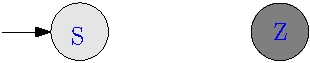
\includegraphics{Images/NdfaREempty.pdf}}
        \end{center} 
    \end{figure}
    
    \item $\bf e = \epsilon$  is converted in:
    \begin{figure}[H]
        \begin{center}
        \resizebox{.1\textwidth}{!}{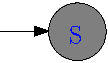
\includegraphics{Images/NdfaREepsilon.pdf}}
        \end{center} 
    \end{figure}
    
    \item  $\bf e = a$ is converted in:
    \begin{figure}[H]
        \begin{center}
        \resizebox{.3\textwidth}{!}{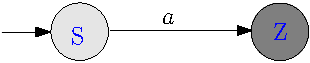
\includegraphics{Images/NdfaRElit.pdf}}
        \end{center} 
    \end{figure}
    
    \item  $\bf e = p\ .\ q$ is converted in:
    \begin{figure}[H]
        \begin{center}
        \resizebox{.7\textwidth}{!}{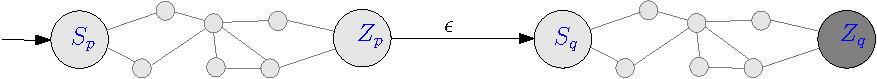
\includegraphics{Images/NdfaREthen.pdf}}
        \end{center} 
    \end{figure}
    
    \item  $\bf e = p + q$ is converted in:
    \begin{figure}[H]
        \begin{center}
        \resizebox{.6\textwidth}{!}{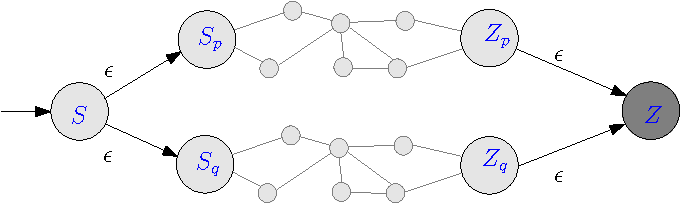
\includegraphics{Images/NdfaREor.pdf}}
        \end{center} 
    \end{figure}
    
    \item  $\bf e = p^*$ is converted in:
    \begin{figure}[H]
        \begin{center}
        \resizebox{.6\textwidth}{!}{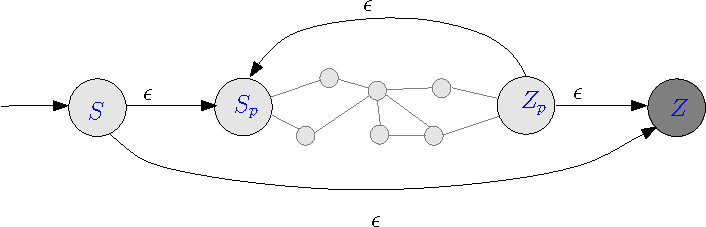
\includegraphics{Images/NdfaREstar.pdf}}
        \end{center} 
    \end{figure}
\end{itemize}

For instance, the regular expression $\bf e = (\epsilon + a^*b)$ would be converted in the NDFA presented in Figure \ref{fig:ndfaT}

\begin{figure}
    \centering
    \resizebox{.8\textwidth}{!}{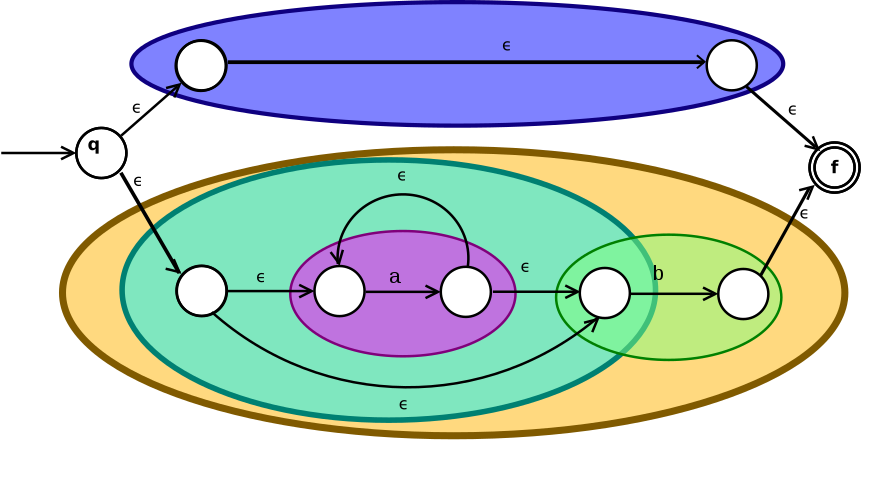
\includegraphics{Images/ndfa.png}}
    \caption{NDFA resulting from $\bf e = (\epsilon + a^*b)$ using Thompson's construction }
    \label{fig:ndfaT}
\end{figure}


\subsubsection{Glushkov's construction algorithm}
Is another well-known algorithm to convert a give RE into a NDFA. Is similar to Thompson's construction, once the $\epsilon$-transitions are removed. Following are the construction steps to create a NDFA that accepts the language $L(e)$ accepted by the RE $e$:

\begin{itemize}
    \item \textbf{Step 1} - linearisation of the expression. Each letter of the alphabet appearing in the expression e is renamed, so that each letter occurs at most once in the new expression $e'$. Let $A$ be the old alphabet and let $B$ be the new one;
    \item \textbf{Step 2a} - the following sets are computed:
    \begin{itemize}
        \item $P(e') = \{\ x \in B\quad |\quad xB^* \cap L(e') \neq \emptyset\ \}$  is the set of symbols which occurs as first letter of a word of $L(e')$. Can be defined inductively:
        
        \begin{flalign*}
            P(\emptyset) & = P(\epsilon) = \emptyset \\
            P(a) & = \{a\} \text{, for each letter $a$} \\
            P(s+t) & = P(s) \cup P(t) \\
            P(s\ .\ t) & = P(s)\ \cup \ \Lambda (s) P(t) \\
            P(s^*) & = P(s)
        \end{flalign*}
        
        
        \item $D(e') = \{\ y \in B\quad |\quad B^*y \cap L(e') \neq \emptyset\ \}$ is the set of symbols that can end a word of $L(e')$. Can be defined inductively with the same rules of $P$ except for the product where
        
        \begin{equation*}
            D(s\ .\ t) = D(t)\ \cup \ D(s)\Lambda(t) 
        \end{equation*}
        
        \item $F(e') = \{\ u \in B^2\quad |\quad B^*uB^* \cap L(e') \neq \emptyset\ \}$ is the set f symbol pair that can occur in words of $L(e')$. Can be defined inductively as follows: 
        \begin{flalign*}
            F(\emptyset) & = F(\epsilon) = F(a) = \emptyset \text{, for each letter $a$} \\
            F(s+t) & = F(s) \cup F(t) \\
            F(s\ .\ t) & = F(s)\ \cup\ F(t)\ \cup\ D(s)P(t) \\
            F(s^*) & = F(s)\ \cup\ D(e)P(e)
        \end{flalign*}
        
    \end{itemize}
    
    \item \textbf{Step 2b} - computes the set $\Lambda = \{\epsilon\} \cup L(e')$, in case the empty word belongs to the language, otherwise $\Lambda = \emptyset$. It can be defined inductively for each RE as following:
    \begin{flalign*}
        \Lambda(\emptyset) & = \emptyset \\
        \Lambda(\epsilon) & = \{\epsilon\} \\
        \Lambda(a) & = \emptyset \text{, for each letter $a$} \\
        \Lambda(s+t) & = \Lambda(s) \cup \Lambda(t) \\
        \Lambda(s\ .\ t) & = \Lambda(s)\ .\ \Lambda(t) \\
        \Lambda(s^*) & = \{\epsilon\} 
    \end{flalign*}
    
    
    \item \textbf{Step 3} - computation of the local language, i.e. the set of words which begin with a letter of $P$, end by a letter of $D$ and whose transitions belong to $F$: 
    \begin{equation*}
        L' = (PB^* \cap B^*D)\ \backslash\ B^* (B^2 \backslash F) B^*
    \end{equation*}
    
    \item \textbf{Step 4} - erasing the delineation, giving to each letter of $B$ the letter of $A$ it used to be.
\end{itemize}

Given the regular expression $\bf e = (a(ab)^*)^* + (ba)^*$, would produce the NDFA in Figure \ref{fig:ndfaG}, without performing Step 4, to perform this step one only needs to remove the index from each symbol in the nodes.

\begin{figure}
    \centering
    \resizebox{.8\textwidth}{!}{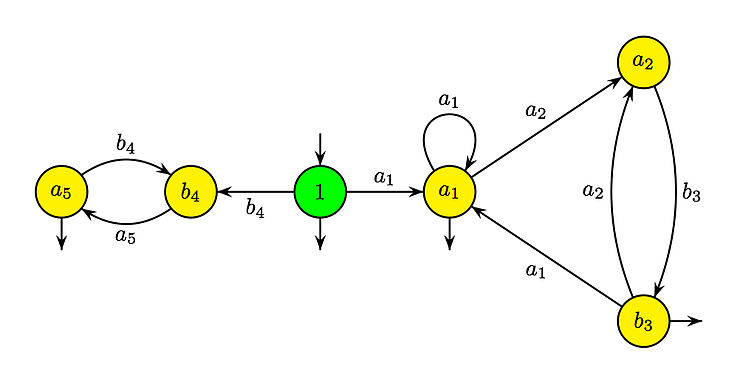
\includegraphics{Images/glushkov.jpg}}
    \caption{NDFA resulting from $\bf e = (a(ab)^*)^* + (ba)^*$ using Glushkov's construction }
    \label{fig:ndfaG}
\end{figure}

\subsubsection{Powerset construction algorithm}
Converts a NDFA into a DFA, which recognize the same formal language. Recall the structure of a NDFA in Section \ref{definitions}, the corresponding DFA has the set of states $Q_D$, where each state corresponds to subsets of $Q_N$. 

The initial state of the DFA is the set $\{q_0\}$ where $q_0$ is the initial state of the NDFA. In case of a NDFA has $\epsilon$-transitions then the initial state of the DFA - $q_{0D}$ - has the initial state of the NDFA - $q_{0N}$ - plus the states reachable from that state through $\epsilon$-transitions - called $\epsilon$-\textit{closure}:
\begin{equation*}
    q_{0D} = q_{0N}\ \cup \ \epsilon\text{-\textit{closure}} \ \{q_{0N}\}
\end{equation*}

Starting from the initial state $q_{0D}$, each new state is computed from another state $S \in Q_D$. It can be defined recursively as:
\begin{itemize}
    \item $q_{0D} \in Q_D$
    \item $qs \in Q_D \Rightarrow \{ d\ |\ (o,y,d) \in \delta_{NDFA} \wedge o \in qs\} \in Q_Dv , \quad \forall y \in \Sigma$
\end{itemize}

The transition function of the DFA maps a state $S$ and the input symbol $y$ to the respective computed state:

\begin{equation*}
    \delta_{DFA} = \cup \{(S,y,D) | D = \{ d\ |\ (o,y,d) \in \delta_{NDFA} \wedge o \in S\}\}, \forall{(y \in \Sigma \wedge S \in Q_D)}
\end{equation*}

Finally, the set of accepting states of the DFA $Z_D$ is the set of states $S \in Q_D$ that contain at least one state that is accepting state in the NDFA:

\begin{equation*}
    Z_D = \{q \in Q_D\ |\ q \cap Z_N \neq \emptyset\}
\end{equation*}

\subsubsection{Kleene's Algorithm}

Kleene's algorithm produces a regular expression from a DFA in the following way.
\begin{enumerate}
    \item It first constructs a graph whose nodes correspond to the states of the automaton and the edges are regular expressions that connect those nodes. 
    \item The initial set of edges contains one edge for each transition in the automaton (labelled with the corresponding literal) plus one edge for each node to itself containing the regular expression $\epsilon$.
    \item It proceeds by applying a variation of the Floyd-Warshall algorithm in order to obtain all paths connecting each of the nodes (summing weights corresponds to concatenation of regular expressions whereas the minimum operation corresponds to alternative ($+$) of regular expressions).
    \item Finally the regular expression equivalent to the original DFA can be obtained as the union ($+$) of the edges which connect the initial state to all final states.
\end{enumerate}